\documentclass[a4paper,10pt]{article}

% Packages
\usepackage[utf8]{inputenc}
\usepackage[frenchb]{babel}
\usepackage{graphicx}
\usepackage{url}
\usepackage{hyperref}
\usepackage{a4wide}
\usepackage{amsmath}
\usepackage{verbatim}
\usepackage{array}
\usepackage{../clrscode3epg}
\renewcommand{\labelenumi}{(\alph{enumi})}

% Style
\parskip=\smallskipamount

% En-têtes
\title{
    \textbf{Structures de données et algorithmes}\\
    Répétition 7: Résolution de problèmes (Partie 1)
}

\author{Gilles \textsc{Louppe} -- \url{http://www.montefiore.ulg.ac.be/~glouppe}}
\date{19 avril 2013}

% Corps
\begin{document}
\maketitle

% http://www.cs.ucsb.edu/~suri/cs130b/NewDivConquer.pdf


\section*{Exercice 1}

Imaginer et donner le pseudo-code d'un algorithme \textit{divide-and-conquer}
permettant de trouver le \textsc{min} et le \textsc{max} dans un tableau $A$ de
longueur $n$ et n'utilisant que $3n/2$ comparaisons. Justifier la complexité de
votre algorithme.


\section*{Exercice 2}

Le problème des tours de Hanoï consiste à déplacer des disques de diamètres différents d'une tour de départ $A$ à une tour d'arrivée $C$ en passant par une tour intermédiaire $B$, et ceci en un minimum de coups, tout en respectant les règles suivantes:

\begin{itemize}
\item on ne peut déplacer plus d'un disque à la fois,
\item on ne peut placer un disque que sur un autre disque plus grand que lui ou sur un emplacement vide.
\end{itemize}

\begin{figure}[h]
    \center
    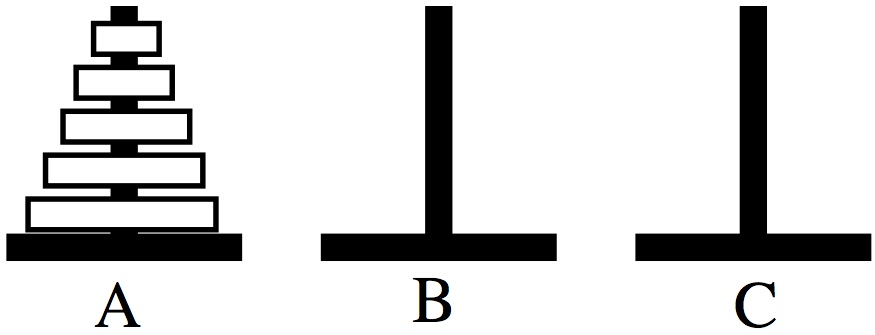
\includegraphics[scale=0.25]{hanoi.jpg}
    \caption{Tours de Hanoi}
\end{figure}

Imaginer et donner le pseudo-code d'un algorithme \textit{divide-and-conquer}
permettant de calculer la séquence de mouvements à effectuer pour déplacer $n$
disques de $A$ vers $C$. Analyser la complexité de votre algorithme.


\section*{Exercice 3}

On souhaite déterminer le zéro $r$ d'une fonction $f(x)$ monotone sur un intervalle $[u, v]$.

\begin{enumerate}
\item Un algorithme par force brute est-il envisageable pour résoudre ce problème?
\item Proposer un algorithme par \textit{divide-and-conquer}.
\end{enumerate}


\section*{Exercice 4}

Soit un ensemble $S$ de points définis dans un plan. L'enveloppe convexe de $S$
est le plus petit polygone convexe incluant tous les points de $S$.

\begin{figure}[h]
    \center
    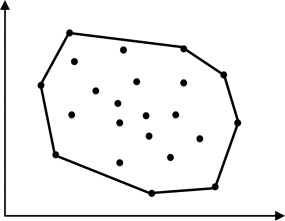
\includegraphics[scale=1.0]{convexhull.jpg}
    \caption{Enveloppe convexe d'un ensemble de points}
\end{figure}

Imaginer et donner le pseudo-code d'un algorithme \textit{divide-and-conquer}
permettant de l'enveloppe convexe de $S$. Analyser la complexité de votre
algorithme.


\section*{Exercice 5}

Soit un ensemble $P = \{p_1, p_2, ..., p_n\}$ de points répartis dans un plan et tels que $p_i = (x_i, y_i)$. Proposer un algorithme qui détermine la distance entre les deux points les plus proches. La mesure de distance utilisée est la distance euclidienne.

% http://en.wikibooks.org/wiki/Algorithms/Divide_and_Conquer#Closest_Pair_of_Points

\section*{Exercice 6}

On souhaite multiplier une série $n$ matrices sous la forme: $$A = A_0 A_1 ... A_{n-1}$$

On note $d_k \times d_{k+1}$ les dimensions de la matrice $A_k$.

\begin{enumerate}
\item L'ordre des multiplications importe t-il?
\item Quelle serait la complexité d'une méthode par force brute pour déterminer le parenthésage optimal à effectuer?
\item Proposer un algorithme par programmation dynamique pour déterminer le parenthésage optimal.
\end{enumerate}


% \section*{Exercice 4}

% On souhaite déterminer le zéro $r$ d'une fonction $f(x)$ monotone sur un intervalle $[u, v]$.

% \begin{enumerate}
% \item Un algorithme par force brute est-il envisageable pour résoudre ce problème?
% \item Proposer un algorithme par \textit{divide-and-conquer}.
% \end{enumerate}

% \section*{Exercice 5}

% % http://www.csc.liv.ac.uk/~ped/teachadmin/algor/d_and_c.html

% Soit un ensemble $P = \{p_1, p_2, ..., p_n\}$ de points répartis dans un plan et tels que $p_i = (x_i, y_i)$. Proposer un algorithme qui détermine la distance entre les deux points les plus proches. La mesure de distance utilisée est la distance euclidienne.

% \section*{Exercice 6}

% On souhaite multiplier une série $n$ matrices sous la forme: $$A = A_0 A_1 ... A_{n-1}$$

% On note $d_k \times d_{k+1}$ les dimensions de la matrice $A_k$.

% \begin{enumerate}
% \item L'ordre des multiplications importe t-il?
% \item Quelle serait la complexité d'une méthode par force brute pour déterminer le parenthésage optimal à effectuer?
% \item Proposer un algorithme par programmation dynamique pour déterminer le parenthésage optimal.
% \end{enumerate}

% \section*{Exercice 1}

% Soit une chaîne de caractères \texttt{S} au format ASCII.

% \begin{enumerate}
% \item Ce codage est-il optimal en termes d'espace mémoire utilisé? Illustrer par un exemple.
% \item Comment réduire la mémoire utilisée?
% \item Proposer un algorithme glouton pour compresser \texttt{S}.
% \item Quel serait le codage de \texttt{S} pour l'exemple proposé en (a)?
% \end{enumerate}

% \section*{Exercice 2}

% % http://people.csail.mit.edu/bdean/6.046/dp/

% Soit une expression booléenne composée des symboles \texttt{true},
% \texttt{false}, \texttt{and} et \texttt{or}. Proposer un algorithme qui
% détermine le nombre de façons de parenthèser l'expression de sorte qu'elle soit
% évaluée à \texttt{true}.

% \section*{Exercice 3 (B. Boigelot, 2009)}

% On considère un terrain de jeu rectangulaire possédant $n.m$ cases organisées en
% $n$ lignes et $m$ colonnes. Des sommes d'argent sont initialement placées sur
% ces cases. Un joueur traverse le terrain à partir du coin supérieur gauche
% jusqu'au coin inférieur droit. A chaque étape de ce trajet, le joueur collecte
% la somme d'argent placée sur la case où il se trouve, et a ensuite le choix de
% se déplacer d'une case soit vers la droite, soit vers le bas (les déplacements
% vers la gauche, vers le haut ou en diagonale sont interdits).

% \begin{enumerate}
% \item Ecrire un algorithme capable de calculer une suite de mouvements qui
% permet au joueur d'atteindre la case inférieure droite en ayant accumulé le
% plus d'argent possible.
% \item Calculer la complexité en temps et en espace de l'algorithme proposé.
% \end{enumerate}

\end{document}
